\section{Proposal}

\subsection{Survey}
This section is supposed to enumerate (at least) \emph{four} references and
briefly summarize the main insight they provided (1 paragraph each). All
references should also be included in the References section that concludes the
report.

\begin{packed_enum}
\item
As Bigtable we understand a distributed storage that is scaleable for a very large size of data. It is stated that many big projects like, Google Earth, Google Analytics and Google Finance, make use of the Bigtable technology. For services in this dimension, such a system has to be stable in latency and should also be able to handle huge data sizes. Bigtable therefore is a technology that meets this high demand needs. It works with clustering, where you can simply add more machines to the system for more demanding applications. \cite{Chang2008}
\item 
In the blog post "New Sql: An Alternative to Nosql and Old Sql For New Oltp Apps" the author Michael Stonebraker talks about Online
Transaction Processing and how it's requirements have changed over the last years. Traditionally a relational DBMS processed customer requests and a data warehouse stored information in a common format to analyse or cross-sell information. In order to convert the OLTP data, a Extract-Transform-and-Load product was used. This system is described by the author as Old OLTP or Old SQL. In contrary New OLTP is needed for Web properties, and mostly defined by two requirements. On the one side, far more OLTP throughput is needed, since the number of interactions per second
sharply rose on web-based applications (e.g. social networks). Another demand is the need for real-time analytics. (e.g. finding surrounding locations of a smartphone).

Following, the author takes a look at Old SQL, NOSql and New SQL systems and how they deal with these requirements. However, Old SQL and NoSQL seem to give no satisfying solution. Since the capabilities of Old SQL may exceed the experience workflow and are incapable of providing real-time analytics.
No SQL on the other side does not fully provide ACID. Which can be problematic for some applications. A solution could be the NewSQL systems. Which offer high performance and scalability as well as preserve ACID properties for transactions. \cite{Stonebraker2011}

\item 
Large-scale infrastructur services need among other things high availabity and perfomance. A way of achivieving this is to use eventual consitency. It is a form of weak consistency and guarantees that if no new updates are to an object, eventually all accesses will return the last updated value. The period where it's not guaranteed that every observer will see the updated value is called inconsitency window. It can be determined based on communication delays, the load of the system and the number of replicas involved in the replication scheme.  
Trading consitency and durability for performance and availabity is not suitable for every application, but can yield advantages such as improving read and write perfomance under highly concurrent conditions and preventing unavailability. It is possible to improves evneutal consitency 
by implementation certain properties, e.g. session-consitency or monotonic read consitency. 

An example for a large scale key-value system is Amazon's Dynamo. \cite{Vogels2009}

\item
In \cite{Stonebraker2010} Michael Stonebraker briefly describes the main differences between SQL databases and NoSQL databases. There are two main categories of NoSQL databases. On the one hand there are "document-style stores", in which a database record consists of key-value pairs and a payload (Examples: MongoDB\footnote{https://www.mongodb.com/} or CouchDB\footnote{http://couchdb.apache.org/}). On the other hand there are "key-value stores", where each record - usually implemented as a distributed hash table - is a key-payload pair (Examples: MemcacheDB\footnote{http://memcachedb.org} or Amazon Dynamo\footnote{https://aws.amazon.com/de/dynamodb/}).

Performance and flexibility are the two main reasons for using a NoSQL system. The author discusses the performance part while talking about OLTP data. The major performance overhead for SQL systems results by using ODBC or JDBC and not SQL on its own. This overhead is caused by logging, locking, latching and buffer management. If you can remove this overhead your database system is faster, not depending if its in a SQL context or not.


\end{packed_enum}

\subsection{System}

We have chosen MongoDB as the basis for our project.

\paragraph{Rationale} Why is this type of system interesting to us? 

As MongoDB is a very widely spread system, it is also very often used in practice. Since all three of us are working in software companies, we are very interested in using and learning real-life technology. We think that MongoDB is most likely to be used in a work place environment. \\ 

Beside from this, we also have a little insight in some of the data structures used there, so we would like to try them out in practice. We think the column- and document- oriented approaches which MongoDB are offering are a huge benefit for our project.

\paragraph{Features} 

\begin{packed_enum}
    \item JSON Like Documents - Data is stored in a flexible way. So it can vary from document to document. This means the data structure is interchangeable anytime without changing the complete database definition.
    \item Document Model - There is a document model which can be used to map objects in application code, so no confusing String handling is necessary for querying.
    \item Ad hoc queries, indexing and real time aggregation - MongoDB is one of the most stable NoSql solutions and for our purpose with its indexing fast enough.
    \item Distributability and Clustering - MongoDB is horizontal scaling and geographically distributeable, so if we would need more computational resources we could provide them easily. 
    \item Free and Open Source - As a completly free project there is a huge community and good documentation, so it's easier to use and learn than other not so well documented systems.\ldots
\end{packed_enum}

\subsection{Application Description}

<<<<<<< HEAD
We decided to write an Android application, which searches a random restaurant from the surrounding area. The idea came up during the time of our bachelor study. We often had problems, choosing a place to have lunch at, since no one wanted to make a final call on where to go.
=======
We decided to write an Android application, which searches a random restaurant from the surrounding area and displays general information about it.
>>>>>>> 863ebf564143f8f5d4272d738d401d3e822edee8

The interface is a simple button, which sends a request to the database system with the current position. As a result, a list of restaurants is returned from which a random selection is made and given to the user. If the user does not like the choice, it is possible to get another random selection by swiping away the location.

The displayed data contains the name, location, homepage-link and opening hours of the restaurant. This data is stored in a database and contains restaurants from Salzburg and it's surroundings. 

For this application a scalable database system with a fast response time is needed. But since the data is not changed by the users, it is not required to fulfill the ACID properties. Hence, a NoSQL database is enough. A document based system makes sense, since the data used already is close to this format, with the location as a unique key for the rest of the information.



\paragraph{Architectural Overview}

Provide an overview on the planned architecture/pipeline of your application.
For example: Programming language(s), 3rd-party libraries/frameworks and their
role in your application pipeline (1 paragraph each), planned/desired
deployment, \ldots

\begin{figure}[H]
	\centering
	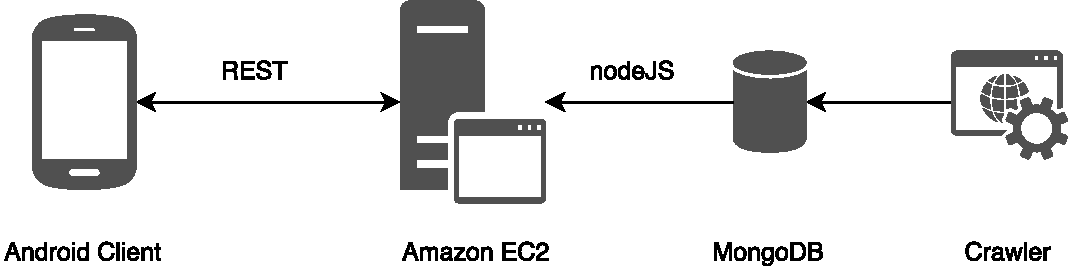
\includegraphics[width=0.8\textwidth]{img/Arch}
	\caption{Architectural Overview}
	\label{fig:Arch}
\end{figure}

As stated in figure \ref{fig:Arch}, the user can interact with the system through an Android application. The data will be fetched in the JSON format through a REST-API. The library used for making API requests is OkHttp\footnote{http://square.github.io/okhttp/}. The data will be cached in a SQLite database using a content provider\footnote{https://github.com/SimonVT/schematic}. The JSON to object conversion will be done by Google's Gson library\footnote{https://github.com/google/gson}. A convenient interface for downloading images and displaying them is Glide\footnote{https://github.com/bumptech/glide}, which we use to display the restaurant's image. 

The data will be fetched from an Amazon EC2 micro server\footnote{https://aws.amazon.com/de/ec2/instance-types/} where we use the free trial. The transmitted data will be in the JSON format and by provided by a nodeJS endpoint\footnote{https://nodejs.org/en/}. To access the MongoDB we will use the provided driver\footnote{https://mongodb.github.io/node-mongodb-native/}.

The database will be filled by a crawler, also written in nodeJS. The crawler will be called periodically by a batch job. 

\paragraph{Experimental Data - Google Places}

\url{https://developers.google.com/places/}

We use the Google Places Api with a filter on restaurants. This api takes a latitude/ longitude pair and a radius as input and returns a list (limited by 20 entries) of restaurants. We will write a JSON Crawler to get more than 20 entries, so we can have a higher area covered by our restaurant list. \\

The data suits our application, because it's easy to parse (JSON) and easy to distribute the data into documents by latitude/longitude pairs. Also our planned data access is by design matching MongoDBs architecture, so we will only have to look up in one document for one join.


\subsection{Roadmap}
\emph{Optional}. Split your project into individual steps and provide a first
roadmap for the project/semester. You may use the \verb|vroadmap| environment
(see \verb|report.tex| for definition):

\begin{vroadmap}
  2018-04-06 & planning finished (research of tools and frameworks) \tabularnewline
  2018-04-13 & seperation of tasks and responsibilities \tabularnewline
  2018-05-04 & first prototype for each part (dummy data possible) \tabularnewline
  2018-05-11 & prototype finished, testing phase starts with real data \tabularnewline
  2018-05-22 & testing finished, fixing of possible bugs, finishing the report \tabularnewline
\end{vroadmap}